
\section{Evaluation}\label{sec:eval}
Our evaluation shows that the proposed out-of-place optimizations substantially reduce total WAF while improving throughput and SSD lifespan 
across various devices (with larger gains on ZNS or FDP), dataset sizes, and benchmarks.  
We focus primarily on write-related metrics, as minimizing flash writes is our main goal.


\subsection{Setup and Methodology}
\module{Hardware setup.}
We evaluate on eight enterprise SSDs from five vendors.
Experiments run on two servers: one with 360~GB DRAM and a 96-core AMD EPYC~9654P, and another with 500~GB DRAM and a 64-core Intel Xeon Gold~6342, both running Ubuntu~24.04~LTS.
The first is used for general tests with 64 worker threads; the second for FDP-enabled SSDs with 32 worker threads.


\module{OLTP benchmarks and DBMS configuration.}
We use two OLTP benchmarks.  
YCSB-A~\cite{DBLP:conf/cloud/CooperSTRS10} (50\% reads, 50\% updates on a fixed-size dataset) is used for performance analysis, and TPC-C is used to assess generality and behavior under growing workloads.  
Both benchmarks target write-intensive OLTP scenarios that become I/O-bound once the dataset exceeds memory.  
\revision[R2.D10]{To reflect realistic OLTP deployments, we set the buffer pool to 5--20\% of the dataset to cache the effective working set~\cite{nvppl,Gray1993DebitCredit,gray1987fiveminuterule}.}  
The WAL size matches the buffer pool unless stated otherwise.

\module{Evaluation method.}
Before each run, we issue \texttt{blkdiscard} to reset SSD mapping state.  
Benchmarks run until cumulative writes reach at least four times the device capacity to ensure steady state~\cite{ssdiq}.  
We report average throughput, DB WAF, SSD WAF, buffer hit ratio, and CPU/memory usage over the final hour, after all configurations have issued comparable cumulative writes.  
DB WAF is total DB-issued writes divided by eviction or checkpoint writes, and SSD WAF is total physical writes (via OCP~\cite{ocp}, when supported) divided by DB-issued writes.

\subsection{Main Performance Result}\label{sec:mainperfresult}
To analyze the impact of each optimization on total WAF, we run YCSB-A (skew = 0.8) across five dataset sizes on a Samsung PM9A3 SSD (894~GB), 
incrementally enabling our optimizations.  
Before introducing GDT, random placement and greedy GC are used.  
When out-of-place writes are enabled, up to 16 open zones are allowed.
The zone size is set to 250~MB prior to aligning the GC unit and to 512~MB afterward, following the configuration inferred from the ZNS-like workload in \cref{sec:gcgranularity} (16 $\times$ 512~MiB = 8~GB in total).
\module{Total WAF.}
As shown in \cref{fig:drilldown:a}, each optimization reduces total WAF across all dataset sizes.
The 160~GB dataset sees a 4.4× reduction (2.33→0.53), while the 800~GB dataset reaches a 7.8× reduction (4.72→0.60) with all optimizations enabled.
Compression contributes the largest improvement by sharply lowering DB WAF.
The NoWA pattern provides the second-largest reduction, with its benefits increasing for larger datasets.

\module{Write drilldown (with compression).}
\cref{fig:drilldown:b} breaks down writes for the 800~GB dataset into user, DWB, DB GC, and SSD GC writes.
In the in-place baseline, DWB dominates, accounting for half of all DB-issued writes.
Switching to out-of-place writes removes DWB but makes DB GC the primary overhead, even increasing total WAF by 1.66×.
Compression with GDT reduces DB GC writes, though SSD GC remains.
Finally, the NoWA pattern together with aligned GC units eliminates SSD GC entirely, leaving user writes dominant and driving total WAF near the compression ratio.


\module{Write drilldown (without compression).}
Compression shrinks the 800~GB dataset to 418~GB, expanding OP space to 53\% of the SSD and reducing the GC valid ratio from 75\% to 14\% (\cref{fig:drilldown:b}).  
This strongly lowers DB WAF and masks the effects of other optimizations, so we omit compression and page packing to isolate their impact and apply the remaining techniques in order.  
As shown in \cref{fig:drilldown:c}, out-of-place writes with all optimizations improve total WAF by 31\% over in-place and by 2.18× over naïve out-of-place.  
GDT reduces DB WAF from 4.02 to 3.36, while NoWA increases it to 3.58 due to compensation writes; however, the resulting drop in SSD WAF outweighs this increase, yielding a net improvement.  
Overall, GDT mitigates DB WAF, while SSD-side optimizations (NoWA and aligning the GC unit) become more impactful without compression.  
\cref{fig:dbsz} further shows that total WAF improves by at least 2× for smaller datasets.

\module{Compression remains highly beneficial.}
Although the other optimizations are effective, compression remains highly beneficial and complements them well.  
Compression provides additional OP space for DB GC, lowering valid ratios by widening the invalidation window~\cite{ssdiq}.  
It also improves deathtime estimation by allowing more writes before GC triggers, giving a larger timestamp window.  
Together, these effects reduce DB WAF during GC.  
Compression also reduces space amplification and often improves throughput, making it recommended whenever datasets are compressible.

\subsection{Performance Drilldown}~\label{sec:drilldown}
To investigate the impact of optimizations on other performance metrics, 
\cref{tab:drilldown} summarizes metrics from the 800~GB dataset experiments shown in \cref{fig:drilldown}.

\begin{table}[t]
\setlength\doublerulesep{0.5pt}
\setlength{\tabcolsep}{0.08cm} % Further reduced column spacing
\small
\centering
\caption{Performance drilldown per proposed optimization (YCSB-A zipf $\theta$ = 0.8, DB size: 800~GB, Samsung PM9A3)}
\label{tab:drilldown}
\begin{tabular}{l | r r r r r r} % adjusted columns
\toprule[1pt]\midrule[0.3pt]
\textbf{Version} & \textbf{OPS} & \textbf{DB} & \textbf{SSD} & \textbf{Logical W.} & \textbf{Physical W.} &  \textbf{Hit} \\
 & \textbf{(K)} & \textbf{WAF} & \textbf{WAF} & \textbf{(Byte/op.)} & \textbf{(Byte/op.)} & \textbf{Ratio} \\
\midrule
in-place & 229 & 2.00 & 2.36 & 1,858 & 4,378 & 0.932 \\
$\rightarrow$ out-of-place & 230 & 4.06 & 1.94 & 3,745 & 7,274 & 0.918 \\
$+$ comp. $+$ pagepack & 380 & 0.62 & 1.95 & 566 & 566 & 0.929 \\
$+$ GDT & 458 & 0.59 & 1.96 & 566 & 1,110 & 0.931 \\
$+$ NoWA & 510 & 0.60 & 1.07 & 567 & 606 & 0.931 \\
$+$ aligning GC Unit & 535 & 0.60 & 1.00 & 567 & 567 & 0.931 \\
$-$ comp. & 328 & 3.58 & 1.00 & 3,364 & 3,364 & 0.927 \\
\midrule[0.3pt]\bottomrule[1pt]
\end{tabular}
\end{table}

\module{Throughput.}
Applying all optimizations reduces total WAF and raises throughput from 229K OPS (in-place writes) to 535K.
Fewer logical writes reduce time spent waiting for I/O~\cite{DBLP:journals/pvldb/LeeAL23,DBLP:journals/pacmmod/WangQYZ25}, 
and lower SSD WAF shortens I/O latency~\cite{ssdiq}, further improving throughput.
Compression with page packing adds further gains by reducing read traffic per operation.

\module{DB WAF.}
For in-place, DB WAF is 2.00 due to double-write buffering.
Out-of-place writes remove this cost, but with the dataset occupying~90\% of SSD capacity and greedy DB GC, DB WAF rises to 4.06.
Compression lowers DB WAF to 0.62 by both giving DB GC additional OP space and reducing the user write volume itself.
GDT-based placement reduces it further to 0.59 by leveraging skew at GC time.
The NoWA pattern slightly increases DB WAF to 0.60 due to compensation writes, but, as shown next, the reduction in SSD WAF outweighs this cost.

\module{SSD WAF.}
In-place writes exhibit SSD WAF~=~2.36, a value that varies across models (see \cref{sec:varyingssds}).
Switching to append-per-zone out-of-place writes reduces this to 1.94, likely because the large sequential write pattern aligns better with SSD internals~\cite{DBLP:conf/fast/MinKCLE12}.
The NoWA pattern further reduces SSD WAF to 1.07.  
While the effect of applying NoWA or GC-unit alignment alone varies by runtime, device model, and workload skew, applying both together consistently eliminates SSD WA, achieving WAF 1.0.

\module{Logical \& physical writes per operation.}
Columns 5--6 of \cref{tab:drilldown} show logical (DB-issued) and physical (SSD-internal) bytes written per operation.
With all optimizations, logical writes drop by 3.27× mainly due to compression; without compression they increase to 1.81×.
Physical writes consistently decrease as SSD WAF approaches 1, eventually converging to logical writes.
Overall, the techniques substantially reduce physically executed writes.

\module{Buffer hit ratio.}
GC I/O can reduce buffer hit ratios because GC reads may evict cached pages.
The largest drop occurs when switching from in-place to out-of-place writes (93.2\%→91.8\%).
Compression improves the valid ratio and restores the hit ratio to 92.9\%; GDT increases it slightly to 93.1\%, since pages read during GC are more likely to be accessed soon (effectively acting as prefetching).
Overall, the optimizations have minimal impact on hit ratio.

\module{CPU overhead.}
In-place writes use 5\% CPU, while out-of-place writes with all optimizations use 8.3\%.
Most overhead comes from securing buffer frames for GC reads.
Since in-place writes already waste ~8\% CPU waiting for synchronous DWB, this extra usage is largely hidden.
Future work will reduce overhead by improving hash-table scans when locating clean frames.

\module{Memory usage.}
We kept the buffer pool size the same across in-place and out-of-place versions to match the amount of user writes per operation.
The out-of-place schemes require extra metadata (\cref{sec:impl}), which is kept in memory,
\revision[R2.D5]{amounting to up to 10.9~GB in the worst case when the device is fully utilized. This bound varies with system configuration, such as compression ratio and zone size.}
If memory is constrained, the system can keep only active metadata in memory and spill the rest to disk, which we leave to future work.

%%%%%%%%%%%%%%%%%%%%%%%%%%%%%%%%%%%%%%%%%%%%%%%%%%%%%%%%%%%%%%%%%%%%%%%%%%%%%%%%%%%%%%%%%%%%%%%%%%%%%%%%%%%%%%%%%%%%%%%%%

\begin{figure}[t]
    \setlength{\abovecaptionskip}{3pt} % space above caption
  \setlength{\belowcaptionskip}{0pt} % space below caption (usually inside float)
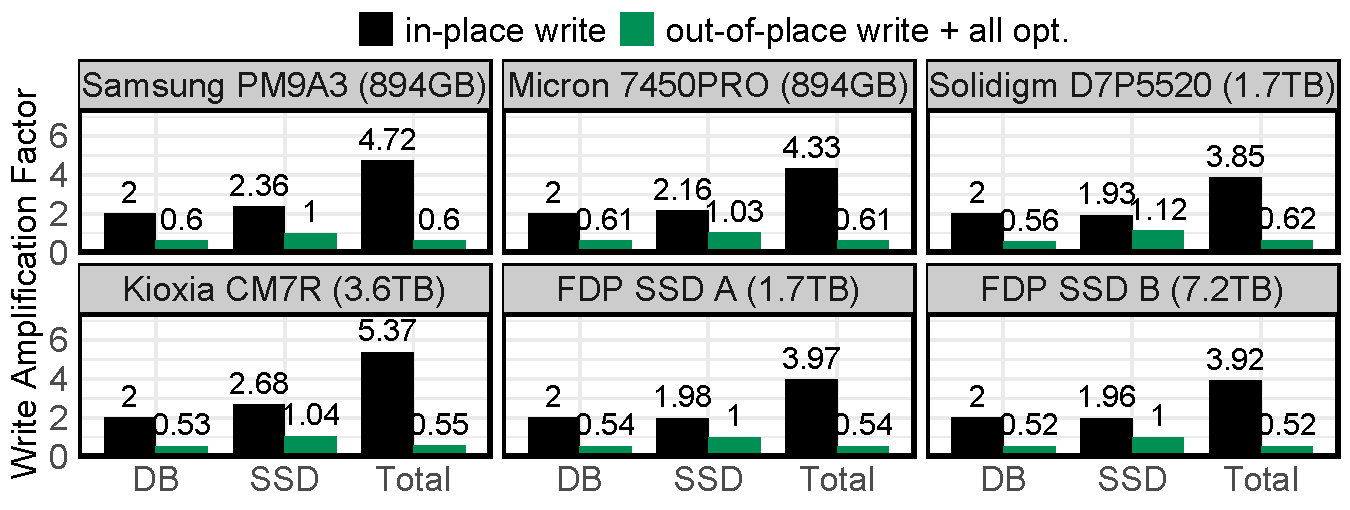
\includegraphics[clip, width=\columnwidth]{figures/varyingssd.pdf}
\caption{\revision{WAF comparison across different SSD models (YCSB-A zipf $\theta$ = 0.8, SSD space 90\% full)}}
\label{fig:varyingssd}
\end{figure}

\subsection{Results Across Various Commodity SSDs}~\label{sec:varyingssds}

\module{Different commodity SSDs.}
To validate our optimizations across SSD models, we repeat the experiment on five additional enterprise SSDs, 
scaling datasets to ~90\% of each device’s capacity (YCSB-A, zipf $\theta$=0.8, 80~GB buffer pool).  
\cref{fig:varyingssd} reports DB, SSD, and total WAF.  
Out-of-place writes consistently reduce total WAF over in-place, with improvements ranging from 6.2× (Solidigm D7-P5520) to 9.76× (Kioxia CM7-R), 
demonstrating robustness across models, vendors, and capacities.  
Larger SSDs exhibit lower DB WAF due to having more OP space (e.g., 7.2\,TB → 752\,GB vs.\ 894\,GB → 94\,GB).  
SSD WAF under out-of-place remains near the optimal value of 1 for all devices except the Solidigm D7-P5520 (1.12), 
which inherently shows slightly higher WAF even on sequential workloads~\cite{ssdiq}.  
In contrast, SSD WAF under in-place ranges from 1.93 to 2.68.  
Overall, the optimizations reliably minimize SSD WAF across devices.

%%%%%%%%%%%%%%%%%%%%%%%%%%%%%%%%%%%%%%%%%%%%%%%%%%%%%%%%%%%%%%%%%%%%%%%%%%%%%%%%%%%%%%%%%%%%%%%%%%%%%%%%%%%%%%%%%%%%%%%%%

\begin{table}[t]
\setlength\doublerulesep{0.5pt}
\setlength{\tabcolsep}{0.14cm} % slightly tighter
\small
\centering
\caption{Throughput comparison on CNS and ZNS SSDs (YCSB-A, zipf $\theta$ = 0.8; capacities: CNS = 894\,GB, ZNS = 951\,GB)}
\label{tab:zns1}
\vspace{-3mm} 
\begin{tabular}{l l l r|r}
\toprule[1pt]\midrule[0.3pt]
\textbf{} & \textbf{Configuration} & \textbf{Used} & \textbf{Logical DB} & \textbf{OPS} \\
\textbf{} & \textbf{} & \textbf{SSD} & \textbf{Size (GB)} & \textbf{(K)} \\
\midrule

\multirow{3}{*}{\makecell{\textbf{in-place vs.}\\\textbf{out-of-place}}}
  & in-place             & CNS & 800  & 156.8 \\
  & oop + all opt.       & CNS & 800  & 322.2 \\
  & oop + comp. + GDT    & ZNS & 800  & 330.3 \\
\midrule

\multirow{2}{*}{\makecell{\textbf{CNS vs. ZNS}\\\textbf{larger DB size}}}
  & oop + all opt.       & CNS & 1,500 & 250.7 \\
  & oop + comp. + GDT    & ZNS & 1,500 & 328.9 \\
  & oop + comp. + GDT    & ZNS & 1,596 & 277.5 \\
\midrule
\midrule[0.3pt]\bottomrule[1pt]
\end{tabular}
\end{table}

\subsection{ZNS and FDP}\label{sec:znseval}

\module{Out-of-place writes benefit CNS, but even more so on ZNS.}
ZNS SSDs offer two key advantages over standard SSDs:  
(1) they naturally maintain SSD WAF~=~1 without requiring NoWA, and  
(2) they expose more usable capacity because no internal OP is needed.  
To evaluate these advantages, we run YCSB-A (zipf $\theta=0.8$) on a 951~GB ZNS SSD and an 894~GB CNS SSD with identical firmware.  
Since CNS cannot report physical writes (no OCP support), we compare throughput instead.  
With an 800~GB dataset (first group in \cref{tab:zns1}), CNS with out-of-place writes doubles the throughput of in-place writes, 
and ZNS further improves throughput---2.1× over CNS in-place and 1.03× over CNS out-of-place.

\module{ZNS vs. CNS with the same dataset size.}
To isolate the benefit of increased usable capacity on ZNS, we evaluate both devices with a 1{,}500~GB dataset (second group in \cref{tab:zns1}).
CNS in-place is omitted since the dataset exceeds its usable capacity.
ZNS outperforms CNS by 31\%, primarily due to lower DB WAF: the additional space reduces the valid ratio during DB GC and avoids NoWA-induced compensation writes.

\module{ZNS vs. CNS at the same fill factor.}
We also compare the devices at the same \emph{relative} fill.
Since 1{,}500~GB on an 894~GB CNS matches the fill factor of 1{,}596~GB on a 951~GB ZNS, we evaluate these configurations (final row in \cref{tab:zns1}).
Here, ZNS outperforms CNS by only $\sim$10\%, much smaller than the previous 31\% gain.
This indicates that most of the benefit stems from ZNS’s larger usable capacity, while removing NoWA overhead yields a smaller incremental gain.

%%%%%%%%%%%%%%%%%%%%%%%%%%%%%%%%%%%%%%%%%%%%%%%%%%%%%%%%%%%%%%%%%%%%%%%%%%%%%%%%%%%%%%%%%%%%%%%%%%%%%%%%%%%%%%%%%%%%%%%%%

\begin{table}[t]
\setlength\doublerulesep{0.5pt}
\setlength{\tabcolsep}{0.14cm}
\small
\centering
\caption{\revision{Effect of FDP on WAFs and throughput (YCSB-A, zipf $\theta$=0.8, 1.6\,TB dataset, FDP SSD A)}}
\label{tab:fdpresults}
\vspace{-3mm} 
\begin{tabular}{l l |rrrr}
\toprule[1pt]\midrule[0.3pt]
\textbf{Configuration} & \textbf{FDP} & \textbf{DB} & \textbf{SSD} & \textbf{Total} & \textbf{OPS} \\
\textbf{} & \textbf{Enabled?} & \textbf{WAF} & \textbf{WAF} & \textbf{WAF} & \textbf{(K)} \\
\midrule
in-place                  & disabled & 2.00 & 1.98 & 3.96 & 437 \\
oop + all opt.            & disabled & 0.57 & 1.00 & 0.57 & 541 \\
oop + all opt. -- NoWA    & enabled  & 0.54 & 1.00 & 0.54 & 553 \\
\midrule[0.3pt]\bottomrule[1pt]
\end{tabular}
\end{table}

%% TODO: fdp soc 확인

\revision[R2.D9]{
\module{SSD WAF = 1 with NoWA vs.\ FDP.}
To isolate the effect of FDP, we evaluate three configurations:
(1) in-place writes;  
(2) out-of-place writes with all optimizations, using NoWA to ensure SSD WAF = 1; and  
(3) out-of-place writes with all optimizations except NoWA, using FDP placement hints to ensure SSD WAF = 1 instead.  
\cref{tab:fdpresults} reports DB WAF, SSD WAF, total WAF, and throughput for these configurations on YCSB-A (zipf $\theta=0.8$) using a 1.6~TB dataset.  
Both out-of-place configurations achieve SSD WAF = 1, whereas in-place writes show SSD WAF = 1.98.  
Without FDP, sustaining SSD WAF = 1 requires the NoWA pattern, whose compensation writes raise DB WAF to 0.57.  
With FDP enabled, placement hints prevent multiplexing directly and further reduce DB WAF to 0.54.  
As a result, total WAF decreases and throughput improves correspondingly.
}


%%%%%%%%%%%%%%%%%%%%%%%%%%%%%%%%%%%%%%%%%%%%%%%%%%%%%%%%%%%%%%%%%%%%%%%%%%%%%%%%%%%%%%%%%%%%%%%%%%%%%%%%%%%%%%%%%%%%%%%%%

\subsection{Effects of Workload Variation}\label{sec:differentworkload}

\begin{figure}[t]
  \setlength{\abovecaptionskip}{3pt} % space above caption
  \setlength{\belowcaptionskip}{0pt} % space below caption (usually inside float)
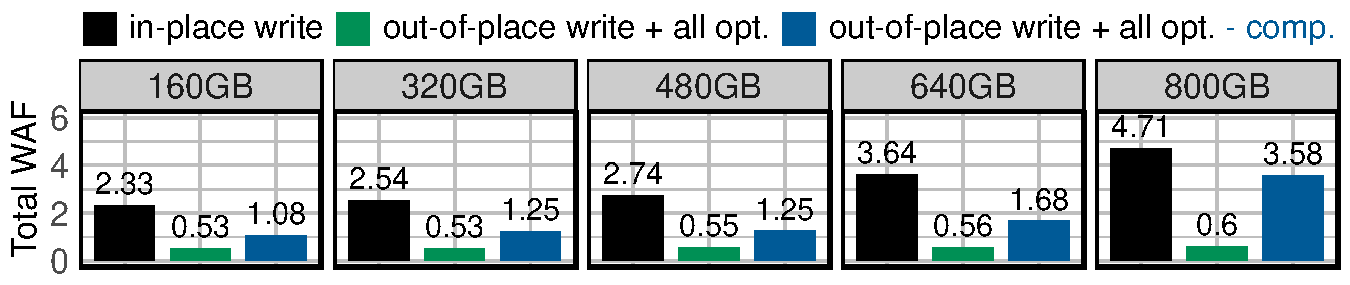
\includegraphics[clip, width=\columnwidth]{figures/dbsz.pdf}
\caption{Total WAF while varying dataset size (YCSB-A zipf $\theta$ = 0.8, Samsung PM9A3)}
\label{fig:dbsz}
\end{figure}
% TODO: show SSD WAF and DB WAF separately, with total WAF?
% for smaller dataset sizes, remove 800GB

\module{Varying dataset size.}
We run YCSB-A (zipfian $\theta = 0.8$) with dataset sizes from 160~GB to 800~GB, setting the buffer pool to 10\% of each dataset.  
\cref{fig:dbsz} reports total WAF for in-place writes, out-of-place writes with all optimizations, and out-of-place writes without compression.  
With in-place writes, total WAF increases from 2.33 (160~GB) to 4.72 (800~GB), whereas out-of-place writes with all optimizations remain low (0.53-0.60).  
Without compression, WAF rises from 1.08 to 3.58 but still stays well below in-place writes.  
The benefits of our optimizations become more pronounced as datasets grow: in-place writes incur rising SSD WAF, while out-of-place writes maintain SSD WAF~=~1.  
Overall, our approach reduces both SSD and DB amplification, even without compression.


% \module{Varying access skew.}  
% We evaluate the effect of workload skewness on total, DB, and SSD WAF by varying the zipfian parameter $\theta$ from 0.0 to 1.0 (\cref{fig:varyskew}).  
% Two key observations emerge.  
% First, workload skewness influences total WAF for both in- and out-of-place writes, but not proportionally.  
% Frequently accessed PIDs are cached in the buffer pool and rarely written to disk except during checkpoints.  
% Thus, tuple-access skew does not directly translate to disk-level skew.  
% For example, $\theta=0.8$ yields the least skewed disk access and the lowest SSD WAF for in-place writes, while $\theta=1$ produces the most skewed disk access and the highest SSD WAF.  
% Second, GDT is more effective for out-of-place writes under highly skewed disk access patterns.  
% As a result, DB WAF is lowest at $\theta=1$, whereas total WAF peaks at $\theta=0.8$, showing an inverse trend compared to SSD WAF for in-place writes.  
% This demonstrates that the total WAF of in-place writes is inversely related to that of out-of-place writes, depending on disk-level access skew rather than tuple-level skewness.  

% \begin{figure}[t]
%     \includegraphics[clip, width=0.75\columnwidth]{figures/varyskew.pdf}
%     \caption{Total WAF while varying skewness (YCSB-A, DB size: 800~GB, Micron 7450 PRO).}
%     \label{fig:varyskew}
% \end{figure}

% \module{Varying WAL file size (i.e., checkpoint frequency).}  
% The previous experiment (\cref{fig:varyskew}) shows that tuple-access skew does not always correspond to disk write skew, 
% since frequently updated PIDs cached in the buffer pool are primarily written only during checkpoints.  
% To further analyze this effect, we vary the maximum WAL file size, which controls checkpoint frequency and thus disk access skew, on a Samsung PM9A3 SSD (\cref{fig:varywal}).  
% In prior experiments, the WAL size matched the buffer pool (80~GB).  
% For comparison, we also run workloads with 10~GB and 640~GB WAL sizes.  
% Our results confirm that smaller WAL sizes produce a more skewed disk access pattern due to more frequent checkpoints, increasing SSD WAF to 2.47 under in-place writes.  
% This higher disk-level skew also amplifies the benefits of out-of-place writes with all optimizations.  
% Conversely, larger WALs trigger fewer checkpoints, producing a less skewed disk access pattern.  
% As a result, the advantage of GDT is reduced, leading to a smaller improvement in total WAF (7.3$\times$), compared to 10~GB WAL size (8.4$\times$).  
% These findings indicate that frequent checkpointing can increase disk access skew and highlight the effectiveness of GDT in such scenarios.

% \begin{figure}[t]
%     \includegraphics[clip, width=\columnwidth]{figures/varywal.pdf}
%     \caption{Total WAF while varying WAL size (YCSB-A, $\theta$ = 0.8, DB size: 800~GB, Samsung PM9A3).}
%     \label{fig:varywal}
% \end{figure}  


% \module{Evaluating with TPC-C.}
% To assess effectiveness beyond YCSB-A, we also run TPC-C~\cite{tpcc}, whose dataset grows over time as new orders are inserted (unlike YCSB-A’s fixed-size workload).  
% We load 15{,}000 warehouses onto FDP SSD~A and run the benchmark for two hours under two configurations: in-place writes and out-of-place writes with all optimizations.  
% \cref{fig:tpcc} plots cumulative flash writes versus cumulative transactions.  
% Within the same runtime, the optimized out-of-place configuration processes 2.45$\times$ more new-order transactions.  
% Conversely, to process the same number of transactions, in-place writes require 7.2$\times$ more flash writes than the optimized configuration.  
% These results demonstrate that our approach remains effective even under different workloads.

\module{Evaluating with TPC-C.}
Beyond YCSB-A, we run TPC-C~\cite{tpcc}, whose dataset grows as new orders arrive (unlike YCSB-A’s fixed size).
We load 15{,}000 warehouses on FDP SSD~A and run two-hour tests with in-place writes and with optimized out-of-place writes.
\cref{fig:tpcc} plots cumulative flash writes versus transactions.
In the same runtime, the optimized out-of-place configuration completes 2.45$\times$ more new-order transactions; for the same transaction count, in-place writes incur 7.2$\times$ more flash writes.
These results show our approach remains effective under a different workload.


\begin{figure}[t]
    \setlength{\abovecaptionskip}{3pt} % space above caption
  \setlength{\belowcaptionskip}{3pt} % space below caption (usually inside float)
    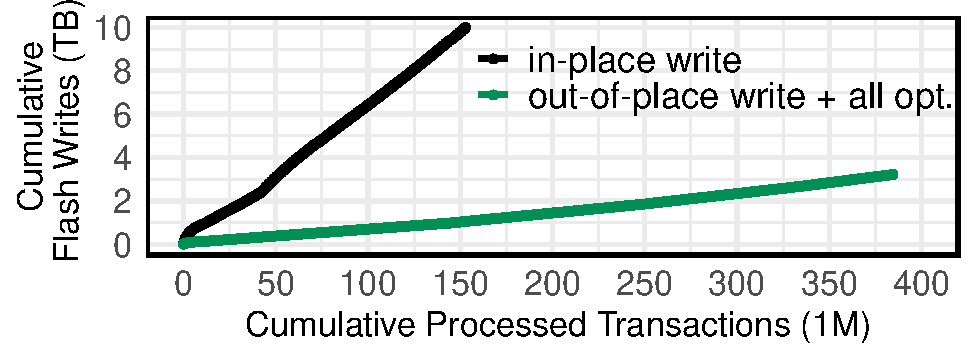
\includegraphics[clip, width=0.75\columnwidth]{figures/tpcc.pdf}
    \caption{Comparison of cumulative flash writes per transaction during the same runtime (TPC-C 15K warehouses ($\approx$ 1.6TB), FDP SSD A).}
     \vspace{-4mm} 
    \label{fig:tpcc}
\end{figure}  


%%%%%%%%%%%%%%%%%%%%%%%%%%%%%%%%%%%%%%%%%%%%%%%%%%%%%%%%%%%%%%%%%%%%%%%%%%%%%%%%%%%%%%%%%%%%%%%%%%%%%%%%%%%%%%%%%%%%%%%%%
